\subsection{Consistency in the case of free electrons}
\begin{figure}
    \centering
    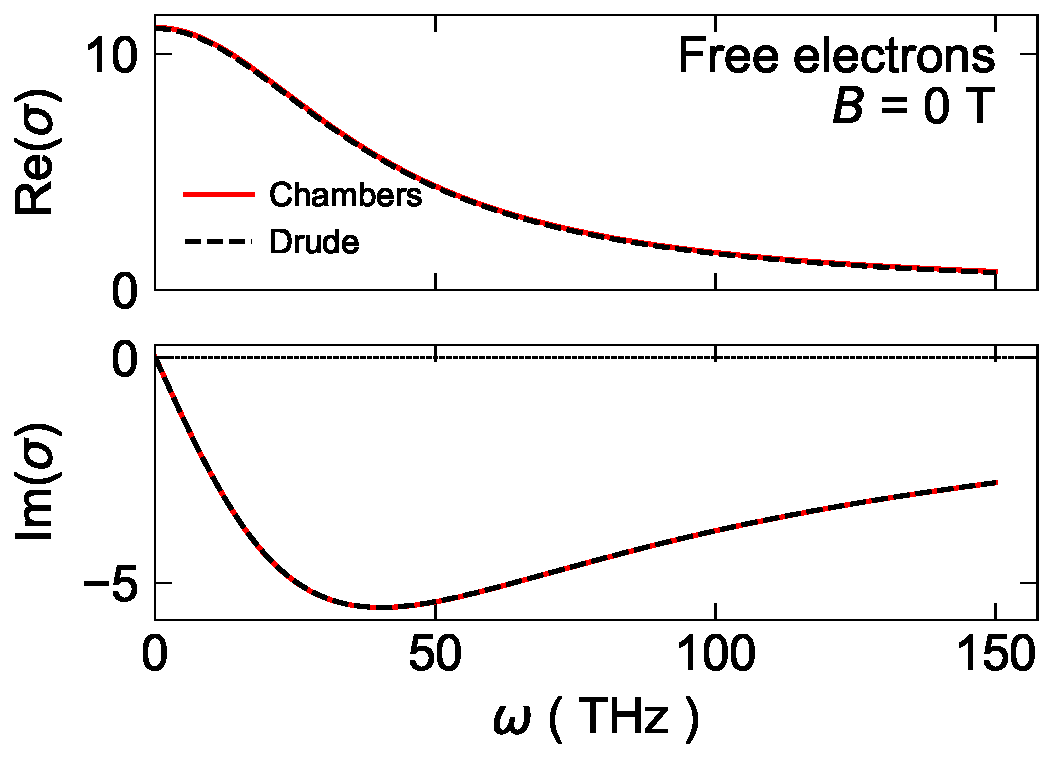
\includegraphics[width=0.7\textwidth]{figures/free_electrons}
    \caption{Agreement of the Drude and Chambers models for free electrons.}
    \label{fig:free_electrons}
\end{figure}

As we explained above, and derived in appendix \textcolor{red}{appendix}, 
the Drude model assumes that the system has particular 'free electron' transport properties. 
This is merely a special case for Chambers' formula, 
and under these assumptions, 
both models are analytically fully equivalent (see appendix \ref{sec:equivalence}).

To make sure our numerical implementation of the new model makes sense, 
we can use this result as a form of validation of our code, on a known case. 
We compared the output of our implementation of Chambers' model in the case of free electrons to the Drude model. 
Figure \ref{fig:free_electrons} shows how the numerical model and the Drude explicit formula agree in this case, \textcolor{red}{for various values of the field B}.

This successful validation test gave us confidence in the soundness of our implementation for further use, 
however this test is not foolproof and we also double-checked the code itself.